%==============================================================================
%== template for LATEX poster =================================================
%==============================================================================
%
%--A0 beamer slide-------------------------------------------------------------
\documentclass[final,32pt]{beamer}

\bibliographystyle{IEEEtran}
%\usepackage[nottoc,numbib]{tocbibind}
\usepackage{cite}


\usepackage[orientation=portrait,size=a1,
            scale=1         % font scale factor
           ]{beamerposter}
           
\geometry{
  hmargin=1.5cm, % little modification of margins
}

%
\usepackage[utf8]{inputenc}

\linespread{1}
%
%==The poster style============================================================
\usetheme{sharelatex}

%==Title, date and authors of the poster=======================================
\title
[Dillon Alexander Heald, University of Cape Town, dillon.heald@gmail.com] % Conference
{ % Poster title
Ultrasonic Directional Audio System
}

\author{ % Authors
\textbf{Author:} Dillon Alexander Heald\inst{1}, \textbf{Supervisor:} A/Prof. A.J. Wilkinson\inst{2}
}
\institute
[University of Cape Town] % General University
{
\inst{1} \textbf{Contact:} dillon.heald@gmail.com
\inst{1,}\inst{2} Dept. of Electrical Engineering, University of Cape Town
}
\date{\today}



\begin{document}
\begin{frame}[t]
%==============================================================================
\begin{multicols}{3}
%==============================================================================
%==The poster content==========================================================
%==============================================================================

\section{Background}
Audible sound for human hearing lies between 20 to 20kHz and conventional loudspeakers perform well at achieving a natural response to match this. However, these speakers cannot easily control where the sound waves go and instead fill the space that the loudspeaker occupies uniformly. Since directivity for a sound source is related to the ratio of wavelength ($\lambda$) to the aperture diameter ($D_{aperture}$) of the source in the form $B_\theta \approx \frac{\lambda}{D_{aperture}}$, apertures much larger than the wavelengths they produce, achieve a high directivity. However, since audible sound has wavelengths between 17 meters to 1.7 centimetres, an infeasible aperture diameter would be required to achieve a high directivity. If instead the transmitted waves are ultrasound, the wavelengths are reduced to between 5.7 to 8.5 millimetres allowing for a smaller aperture of a few centimetres to achieve a high directivity.
\subsection{Problem statement}
Since these ultrasonic waves are inaudible, they need to be translated down in frequency to the human hearing range. This can be done by exploiting a property of air acting as a nonlinear medium when propagating ultrasonic waves. According to Berktay's far-field solution \cite{berktay_1965}, the secondary pressure wave is proportional to the second time derivative of the primary pressure wave squared. A simplified form of Berktay's far-field solution ignoring medium related constants is shown in equation \ref{eqn:berktayRelationship} where $p_1 (t)$ and $p_2 (t)$ represent the primary (input) and secondary (output) sound pressure waves respectively when an ultrasonic wave is propagated in a medium.
\begin{equation}
    p_2(t) \propto \frac{\partial^2}{\partial t^2}p_1^2(t)
    \label{eqn:berktayRelationship}
\end{equation}
The non-linearity caused by the squaring shown in equation \ref{eqn:berktayRelationship} creates sum and difference frequencies when sinusoidal waves are applied. Since the sinusoidal waves are in the ultrasonic range, the sum produces higher ultrasonic frequencies while the difference produces lower audible baseband frequencies.\\
This translation from ultrasonic to audible frequencies is known as self-demodulation and causes the ultrasonic beam itself to become a virtual loudspeaker which artificially extends the aperture diameter beyond the physical bounds of the radiating transducers, thus improving directivity of the audible sound.

\section{Simulation \& Theory}
The purpose of the simulations were to identify what the main signal processing factors are when producing a directional audio system. To do so, the audible signal had to be generated and the inverse transfer function of the environment applied through pre-processing to overcome the operations the environment performs on the pressure wave. Finally, the approximate transfer function of the environment (equation \ref{eqn:berktayRelationship}) is applied along with appropriate filtering to mimic the human hearing range. The simulations created relevant signals in Julia and applied the mathematical operations shown in equation \ref{eqn:inverseApply} for pre-processing. The pre-processed signal features a double integral and square-root operation to overcome the operations imposed by the environment shown in equation \ref{eqn:berktayRelationship}. Letting $p_1(t) = \sqrt{\phi(t)}sin(\omega_c t)$ and applying it to the relationship as shown in equation \ref{eqn:berktayRelationship} becomes $\frac{1}{2} \left(\phi(t)-\phi(t)cos(2\omega_c t) \right)$ due to the squaring term, thus producing the sum (ultrasonic) and difference (baseband) frequencies as expected. The results showed a sample for sample match between the original signal and its self-demodulated difference frequency output in an ideal environment.
\begin{equation}
        \iint \sqrt{\phi(t)} dt^2
        \label{eqn:inverseApply}
\end{equation}
\section{Design}
The design of the directional audio system involves many individual subsystems to achieve the directional audio beam. Each of these subsystems are shown in figure \ref{fig:highleveldesign} where the flows between each component are illustrated. 
The pre-processing, mixer and amplifier designs and simulations are trivial, thus are described further in the written paper of this poster. The parametric acoustic array design and simulation involved many packing simulations and arrived at the chosen design shown in figure \ref{fig:sqr_elem}. The resulting beam pattern simulations performed in Julia via 2DFFT are shown in figure \ref{fig:sqr_elem_topBeam} and \ref{fig:sqr_elem_3Dbeam}. The chosen array design resulted in a large main lobe with 4 major side lobes surrounding it. These side lobes occur due to the spacing between transducers forming inconsistencies in the aperture. Several revisions of the array PCB were designed and resulted in the monolithic square packed circuilar aperture shown in figure \ref{fig:sqr_done}. 
\begin{figure}[h]
    \centering
    \includegraphics[width=0.8\columnwidth]{Figures/Design/HighlevelSystemDesign (1).png}
    \caption{High level system design for the directional audio system}
    \label{fig:highleveldesign}
\end{figure}
\begin{figure}[h!]
\centering

    \begin{minipage}{0.49\columnwidth}
    \centering
    \includegraphics[width= 0.68\textwidth]{Figures/Design/arraySim/SquarePacking_r0.8_R4.5.png}
    \caption{Packed elements to be modelled}
    \label{fig:sqr_elem}
    \end{minipage}\hfill
    \begin{minipage}{0.49\columnwidth}
    \centering
    \includegraphics[width=1.1\textwidth]{Figures/Design/arraySim/2dbeamzoom.png}
    \caption{Approximate beam shape (Bore-sight view)}
    \label{fig:sqr_elem_topBeam}
    \end{minipage}
    
\end{figure}


\begin{figure}[ht!]
    \centering
    \includegraphics[width=\columnwidth]{Figures/Design/arraySim/3dbeamcolzoomier.png}
    \caption{Approximate beam shape of square packed ultrasonic transducer array (3D view)}
    \label{fig:sqr_elem_3Dbeam}
\end{figure}

\begin{figure}[ht!]
    \centering
    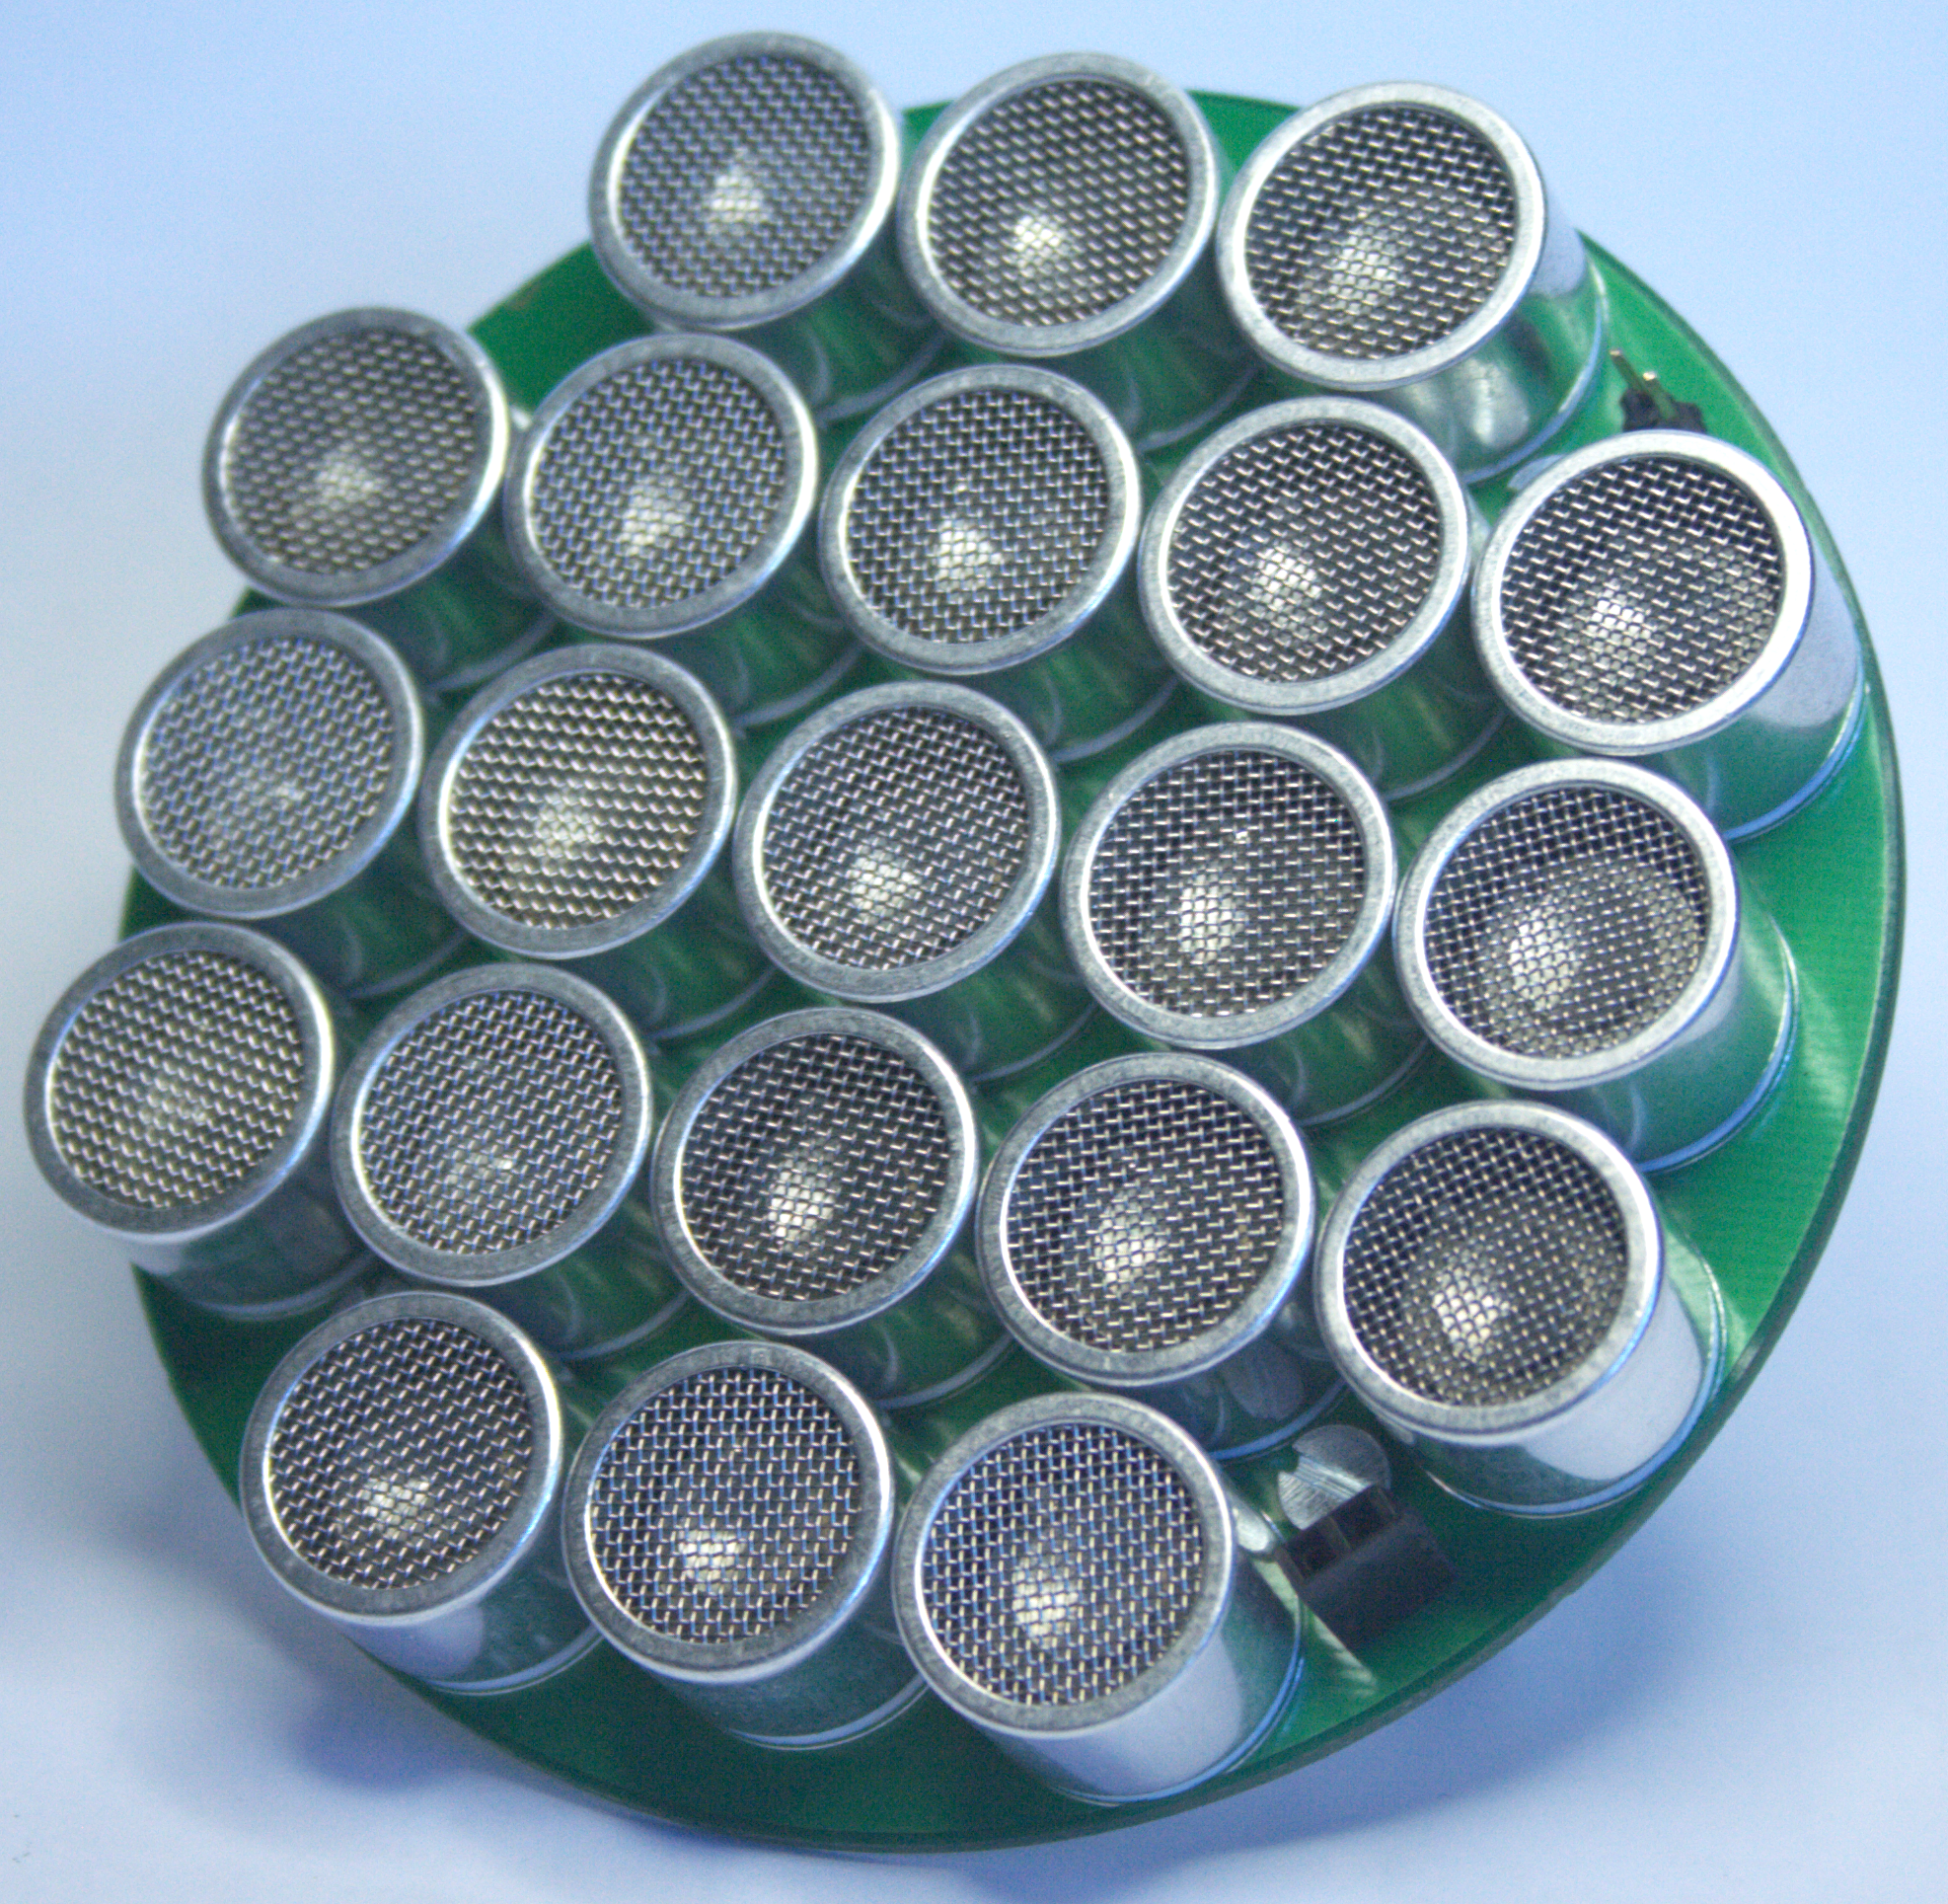
\includegraphics[width=\columnwidth]{Figures/pcbdoneFrontdiag.png}
    \caption{Front side of populated PCB}
    \label{fig:sqr_done}
\end{figure}

\begin{figure}[ht!]
    \centering
    \includegraphics[width=0.7\columnwidth]{Figures/Test/Test_setup.png}
    \caption{The test setup for testing directivity}
    \label{fig:test_setup}
\end{figure}

\begin{figure}[ht!]
    \centering
    \includegraphics[width=\columnwidth]{Figures/Test/original_sig_fft_amp.png}
    \caption{The result for directivity testing}
    \label{fig:test_direct}
    \includegraphics[width=\columnwidth]{Figures/Test/SQRT_fft_sig_straighton.png}
    \caption{The result for distortion testing}
    \label{fig:test_distortion}
\end{figure}

%\begin{figure}[ht!]
%    \centering
%    \includegraphics[width=\columnwidth]{Figures/Test/SQRT_fft_sig_straighton.png}
%    \caption{The result for distortion testing}
%    \label{fig:test_distortion}
%\end{figure}


\section{Implementation \& Testing}
The implementation of the designed array is shown in figure \ref{fig:sqr_done} in the form of a circular PCB with square packed elements. This array was connected to the other subsystems shown in figure \ref{fig:test_setup} and tested to identify how directive and distorted its self-demodulated baseband audio beam is. The test setup for this is shown in figure \ref{fig:test_setup} where the speaker's aperture is rotated through $180^\circ$ to illustrate the approximate directivity of the beam. During the implementation it was discovered that the integration shown in equation \ref{eqn:inverseApply} to counteract the differentiation from equation \ref{eqn:berktayRelationship} was unnecessary as a stronger signal to noise ratio was achieved without this integration during implementation. Therefore, only square-root pre-processing was used in testing with large carrier amplitude modulation.
\section{Result and discussions}
The result for directivity testing revealed a sharp increase in sound pressure level intensity as the ultrasonic beam crossed the microphone. This is compared to a traditional loudspeaker in the paper which features little change as the speaker sweeps through the $180^\circ$ arc. Figure \ref{fig:test_direct} shows the unfiltered sweep for the directional beam along with the FFT of this recording. The FFT shows a strong presence of the 2.5 kHz test tone along with 1st and 2nd harmonics. The paper does further investigation by filtering the recordings for the fundamental test tone, 1st and 2nd harmonics at 5 and 7.5 kHz respectivley. It was found that as the frequency of these harmonics increased, the directivity increased as well which is demonstrated with the artificially produced illustration in figure \ref{fig:approxbeamfreq}.\\
The distortion results for the directional speaker are shown in figure \ref{fig:test_distortion} and demonstrate a large presence of the 1st harmonic of the test tone. This was likely due to the previously mentioned relationship between beam angle and frequency shown in figure \ref{fig:approxbeamfreq} since when the same test was performed with the beam slightly off $0^\circ$ relative to the microphone, the 2.5 kHz fundamental tone was stronger and represented an FFT similar to that shown in figure \ref{fig:test_direct} for the directionality tests.

\begin{figure}[ht!]
    \centering
    \includegraphics[width=0.8\columnwidth]{Figures/Test/beamangle_illustration (1).png}
    \setlength{\belowcaptionskip}{-10pt}
    \caption{Approximate relationship between beam angle and frequency for the directional speaker}
    \label{fig:approxbeamfreq}
\end{figure}


\section{Discussion \& Conclusion}


The simulations proved that the square-root AM pre-processing of the signal would result in an audible baseband signal once applied to the environment due to Berktay's approximation shown in equation \ref{eqn:berktayRelationship}. This was then followed by the design of the directional audio system which would implement the simulated signal chain. This system involves pre-processing baseband audio with a double integral and square-root operation, followed by modulating the signal with a 40 kHz carrier and amplifying the signal before being emitted out of a specially designed ultrasonic transducer array. Notable effort was put into the design and simulation of the transducer array to achieve an efficient aperture for producing the directional audio beam.\\
During implementation, it was identified that the integration shown in equation \ref{eqn:inverseApply} was not necessary and performing the integration during pre-processing simply reduced the signal to noise ratio and thus was omitted. The test setup for directivity was then described and involves the transducer array being swept through a $180^\circ$ arc and recorded with a microphone positioned some distance away. The distortion testing involved recording the sound produced by the speaker when facing the microphone and resulted in a stronger 1st harmonic than the fundamental of 2.5 kHz. When shifting the beam off axis to the microphone, a stronger 2.5 kHz tone was recorded. This resulted in the conclusion that the beam is more directive for higher frequency components, thus its harmonics are stronger when the microphone is in the centre of the beam.
\subsection{Future recommendations}
%A future implementationof this system could explore alternative modulation techniques and identify which techniqueresults in a lowered cost implementation with a higher quality audio beam.
In future implementations, the directional audio system could benefit from an investigation into alternative modulation techniques to achieve higher quality audio.
%The frequency response and transfer function of the transducer could be measured andimported into simulations, allowing for a more realistic signal simulation of the entire signalchain. This could help in discovering what modulation and pre-processing techniques workbest with the limited bandwidth of the transducers in use.
Additionally, characterisation of the transducers transfer functions could be measured and implemented in the design to aid the investigation into working with the limited bandwidth of these transducers.
%The transducer array designed in this project produced a relatively strong directivity comparedto a traditional speaker but struggled to produce significant sound pressure levels. A futureimprovement could investigate alternative transducers or even larger scale transducer arraysand how they effect the resultant output power of the system. This improvement may wantto investigate the use of alternatively shaped modular PCBs for the array as the solution inthis project is not easily scalable.
Regarding the array itself, the designed array could benefit from additional output power by redesign for a more scalable array with more transducers.

%A future implementation may wantto consider placing the array on a platform with remotely controllable rotation increments.Then capturing recordings at set angles relative to the microphone and processing this into abeam pattern plot for a more conventional directivity result.
Finally, the directivity testing results were limited due to lack of resources and thus could be improved by making use of a motorised rotating platform to finely control the angle of the incident beam, thus producing a more conventional beam pattern plot.
%==============================================================================
%==End of content==============================================================
%==============================================================================

%--References------------------------------------------------------------------

\subsection{References}
\bibliography{Bibliography/Bibliography}
%\begin{thebibliography}{99}

%\bibitem{ref1} J.~Doe, Article name, \textit{Phys. Rev. Lett.}

%\bibitem{ref2} J.~Doe, J. Smith, Other article name, \textit{Phys. Rev. Lett.}

%\bibitem{web} \url{http://www.google.pl}

%\end{thebibliography}
%--End of references-----------------------------------------------------------

\end{multicols}

%==============================================================================
\end{frame}
\end{document}
